\documentclass[10pt, leqno]{amsart}

\usepackage{algorithm}
\usepackage[noend]{algpseudocode}
\usepackage{amsfonts}
\usepackage{amsmath}
\usepackage{amssymb}
\usepackage{amsthm}
\usepackage[backend=biber, citestyle=numeric-comp, bibstyle=ieee]{biblatex}
\usepackage{changepage}
\usepackage{enumitem}
\usepackage{fancyhdr}
\usepackage{fontspec}
\usepackage{fullpage}
\usepackage[hidelinks]{hyperref}
\usepackage{marvosym}
\usepackage{mathtools}
\usepackage[]{mdframed}
\usepackage{physics}
\usepackage{tabularx}
\usepackage[skins]{tcolorbox}
\usepackage{thmtools}

\usepackage{tikz-3dplot}
%\usetikzlibrary{angles, calc, cd, quantikz, quotes, patterns}
\usetikzlibrary{angles, calc, cd, quotes, patterns}
\usepackage{titlesec}
\usepackage{wasysym}

\usepackage{tikz-cd}

\usepackage{bookmark}
\usepackage[nameinlink]{cleveref}

\titleformat{\section}[runin]{\normalsize\bfseries}{\thesection}{1em}{}[]
\titleformat{\subsection}[runin]{\normalsize\bfseries}{\thesubsection}{1em}{}[]
\titleformat{\subsubsection}[runin]{\normalsize\bfseries}{\thesubsubsection}{1em}{}[]

\addbibresource{notes.bib}

\theoremstyle{definition}
\newtheorem{theorem}{Theorem}[section]
\newtheorem{conjecture}{Conjecture}[section]
\newtheorem{definition}{Definition}[section]
\theoremstyle{remark}
\newtheorem{problem}[theorem]{Problem}
\newtheorem{lemma}[theorem]{Lemma}
\newtheorem{remark}[theorem]{Remark}
\newtheorem{observation}[theorem]{Observation}
\newtheorem{example}[theorem]{Example}
\newtheorem{corollary}[theorem]{Corollary}

\renewcommand{\qedsymbol}{\(\blacksquare\)}

\setlength{\parindent}{0pt}

\renewcommand{\theequation}{\thesection.\arabic{equation}}

\DeclareMathOperator{\controrot}{CR}
\DeclareMathOperator{\expectation}{E}
\DeclareMathOperator{\gf}{GF}
\DeclareMathOperator{\qft}{QFT}
\DeclareMathOperator{\rk}{rk}
\DeclareMathOperator{\defect}{def}
\DeclareMathOperator{\swapgate}{SWAP}
\DeclareMathOperator{\che}{CHE}
\DeclareMathOperator{\poly}{poly}
\DeclareMathOperator{\Span}{Span}
\DeclareMathOperator{\diag}{diag}

\newcommand{\djk}{\delta_{j, k}}
\newcommand{\tlk}{\tilde{\lambda_k}}

\newcommand{\evalat}[2]{\left.{#1}\middle|\right._{#2}}

% SOURCE: https://tex.stackexchange.com/questions/296151/double-head-and-hook-arrow
\newcommand{\hookdoubleheadrightarrow}{%
  \hookrightarrow\mathrel{\mspace{-15mu}}\rightarrow
}

\newtcolorbox{edgebox}{enhanced, colback=white, frame code={%
\draw[very thin] (frame.north west) -- ($(frame.north west) + ( 0.5, 0)$);
\draw[very thin] (frame.north west) -- ($(frame.north west) + (0, -0.5)$);
\draw[very thin] (frame.south east) -- ($(frame.south east) + (-0.5, 0)$);
\draw[very thin] (frame.south east) -- ($(frame.south east) + (0,  0.5)$);
}}

\AtEveryBibitem{%
  \clearfield{journaltitle}%
  \clearfield{date}%
  \clearfield{volume}%
  \clearfield{pages}%
  \clearfield{publisher}%
  \clearfield{number}%
  \clearfield{journaltitle}%
}

\newcommand{\commentcmd}[1]{}

\newcommand{\draftcomment}[2]{\textcolor{#1}{#2}}
\newcommand{\draftcommenttodo}{\textcolor{red}{ TODO }}
\newcommand{\draftcommentdone}{\textcolor{green}{ DONE }}
%\newcommand{\draftcommenttodo}{}
%\newcommand{\draftcommentdone}{}

\newcolumntype{L}[1]{>{\raggedright\arraybackslash}p{#1}}
\newcolumntype{C}[1]{>{\centering\arraybackslash}p{#1}}

\begin{document}
    \begin{mdframed}
        \textsc{Seminar on Measure and Integration Theory} \hfill valentinpi\\
        Freie Universität Berlin \hfill February 18, 2025\\
        Winter Term 2024-25
    \end{mdframed}

    \section*{Presentation Notes on: Measure Decomposition Theorems}

    The general aim of this presentation is to discuss decomposition theorems for measures. Decomposition is an often occuring pattern in mathematics, as it makes objects easier to grasp and compare with one another. Almost all of the contents of these notes can be found in \cite[pp. 71-76, pp. 113-118]{Fonseca}. Throughout this document, assume that \((X, \mathfrak{M})\) is a measurable space. We quickly recall the major result of the first presentation on the comparison of measures, the Radon-Nikodym theorem, here in the less general version.

    \begin{theorem}[{Radon-Nikodym I \cite[pp. 56-59]{Fonseca}}] \label{thm:radon_nikodym_i}
        Let \(\mu, \nu\colon \mathfrak{M} \to [0, \infty]\) be two measures with \(\mu\) \(\sigma\)-finite and \(\nu \ll \mu\). Then there is a measurable \(u\colon X \to [0, \infty]\) with
        \begin{align}
            \nu(\cdot) = \int_\cdot \, u \, d\mu,
        \end{align}
        which is unique up to a set of \(\mu\)-measure zero.
    \end{theorem}

    We will use this result later.

    \section{Decomposition Theorems for Measures}

    \subsection{Auxiliary Measures} We recall the following definitions.
    \begin{definition}[{\cite[p. 55]{Fonseca}}] \label{def:basic_definitions}
        Let \(\mu, \nu\colon \mathfrak{M} \to [0, \infty]\) be two measures.
        \begin{enumerate}[label=(\roman*), wide]
            \item \(\nu\) is said to be \emph{absolutely continuous} wrt. \(\mu\), \(\nu \ll \mu\), if for any \(E \in \mathfrak{M}\), \(\mu(E) = 0 \rightarrow \nu(E) = 0\).
            \item \label{def:basic_definitions_2} \(\mu, \nu\) are said to be \emph{mutually singular}, \(\nu \perp \mu\), if there are disjoint \(X_\mu, X_\nu \in \mathfrak{M}\) with \(X = X_\mu \cup X_\nu\) and \(\mu(E) = \mu(E \cap X_\mu)\), as well as \(\nu(E) = \nu(E \cap X_\nu)\) for any \(E \in \mathfrak{M}\).
            \item \(\nu\) is said to be \emph{diffuse} wrt. \(\mu\), if for any \(E \in \mathfrak{M}\), \(\mu(E) < \infty \rightarrow \nu(E) = 0\).
        \end{enumerate}
    \end{definition}

    Recall the motivation for the definition of absolute continuity: If \(\nu \ll \mu\), then
    \begin{align}
        \lim_{\mu(E) \to 0} \nu(E) = 0
    \end{align}
    with the formal statement on \cite[pp. 55-56]{Fonseca}. Mutual singularity relates to the abiliy to single out the actions of each measure on parts of a partition, similar to how the action of a matrix can be separated by considering the action on each subspace induced by a single basis element. Diffuseness relates to \(\mu\) diffusing the zeroing-actions of \(\nu\), thus, the order of \(\nu\) and \(\mu\) should be switched in the definition, but it is convention to keep it this way. Further recall, that we can also write the equations in \Cref{def:basic_definitions} \ref{def:basic_definitions_2} as
    \begin{align}
        \mu = \mu|_{X_\mu} \text{ and } \nu = \nu|_{X_\nu}
    \end{align}
    by invoking the standard notation for restricting a measure by cutting a given set before the measurement.
    
    \phantom{}
    
    Based on these three definitions, we introduce three auxiliary measures for any given measure.

    \begin{definition} \label{def:basics_on_measure_relations}
        Let \(\mu, \nu\colon \mathfrak{M} \to [0, \infty]\) be two measures. We define the following three set functions:
        \begin{align}
            \nu_{ac}&\colon \mathfrak{M} \to [0, \infty], E \mapsto \max\left\{\int_E u \, d\mu \, \middle\vert \, u\colon X \to [0, \infty] \text{ measurable} \land \int_{E'} u \, d\mu \leq \nu(E') \, \forall \, \mathfrak{M} \ni E' \subseteq E\right\}\\
            \nu_s&\colon \mathfrak{M} \to [0, \infty], E \mapsto \max\{\nu(E') \mid \mathfrak{M} \ni E' \subseteq E, \mu(E') = 0\} \\
            \nu_d&\colon \mathfrak{M} \to [0, \infty], E \mapsto \max\{\nu(E') \mid \mathfrak{M} \ni E' \subseteq E, \mu(E'') = \infty \, \forall \, \mathfrak{M} \in E'' \subseteq E', \nu(E'') > 0\}
        \end{align}
    \end{definition}

    The indices \(ac\), \(s\) and \(d\) refer to \emph{absolutely continuous}, \emph{singular} and \emph{diffuse}, respectively. The function \(\nu_{ac}\) has been used in the previous presentation on the comparison of measures as a tool for proving \Cref{thm:radon_nikodym_i}. % the Radon-Nikodym theorem \cite[pp. 56-64]{Fonseca}.

    \begin{edgebox}
        \begin{lemma}[{\cite[pp. 13-14]{Fonseca}}] \label{lem:special_measure_1}
            Let \(\mu\colon \mathfrak{M} \to [0, \infty]\) be a measure, \(\mathfrak{N} \subseteq \mathfrak{M}\) be closed under finite unions and \(\emptyset \in \mathfrak{N}\). Then
            \begin{align}
                \nu\colon \mathfrak{M} \to [0, \infty], E \mapsto \max\{\mu(E \cap F) \mid F \in \mathfrak{N}\}
            \end{align}
            is well-defined and a measure.
        \end{lemma}
    \end{edgebox}

    \begin{lemma} \label{lem:auxiliary_functions_lemma}
        The following statements hold.
        \begin{enumerate}[label=(\roman*), wide]
            \item \label{lem:auxiliary_functions_lemma_1} \(\nu_{ac}\), \(\nu_s\) and \(\nu_d\) are well-defined and measures.
            \item \label{lem:auxiliary_functions_lemma_2} \(\nu_{ac} \ll \mu\).
            \item \label{lem:auxiliary_functions_lemma_3} If \(\nu_s\) is \(\sigma\)-finite, then there exists some \(X_s \in \mathfrak{M}\), s.t.
            \begin{align}
                \mu(X_s) = 0 = \nu_d(X_s) \text{ and } \nu_s(E) = \nu(E \cap X_s)
            \end{align}
            for all \(E \in \mathfrak{M}\). Also, \(\nu_s \perp \mu\) and \(\nu_s \perp \nu_d\).
            \item \label{lem:auxiliary_functions_lemma_4} \(\nu_{d}\) is diffuse wrt. \(\mu\).
        \end{enumerate}
    \end{lemma}

    \begin{proof}
        \ref{lem:auxiliary_functions_lemma_1} \ref{lem:auxiliary_functions_lemma_2} As for the properties of \(\nu_{ac}\) mentioned, we should have discussed them in a previous presentation, so we do not do this here again. See \cite[pp. 56-59]{Fonseca} for the proofs. For the record, we recall the general idea: \(\nu_{ac}(\emptyset) = 0\) follows from the definition and the \(\sigma\)-additivity can be shown directly using the definition and the supremum. The well-definedness is then shown by constructing an increasing sequence of measurable functions \(\{u_n\colon X \to [0, \infty]\}_{n \in \mathbb{N}_{\geq 1}}\) using the definition of \(\nu_{ac}\) and employing the Lebesgue monotone convergence theorem.

        \ref{lem:auxiliary_functions_lemma_1} Observe by definition, that for any \(E \in \mathfrak{M}\),
        \begin{align}
            \nu_s(E) = \max\{\nu(E \cap F) \mid F \in \mathfrak{N}\}
        \end{align}
        with \(\mathfrak{N} \coloneqq \{F \in \mathfrak{M} \mid \mu(F) = 0\}\). Applying \Cref{lem:special_measure_1} gives the statement, including the well-definedness. We have similarly, that
        \begin{align}
            \nu_d(E) = \max\{\nu(E \cap F) \mid F \in \mathfrak{N}\}
        \end{align}
        for \(\mathfrak{N} \coloneqq \{F \in \mathfrak{M} \mid \mu(F') = \infty \, \forall \, \mathfrak{M} \in F' \subseteq F, \nu(F') > 0 \}\). Observe, that for \(F, F' \in \mathfrak{N}\), \(\mathfrak{M} \ni F'' \subseteq F \cup F'\) with \(\nu(F'') > 0\) and wlog. \(\nu(F'') \geq \nu(F'' \cap F) > 0\), \(\mu(F'') \geq \mu(F'' \cap F) = \infty\). The other possible cases are analogous. Applying \Cref{lem:special_measure_1} again gives the statement.

        \ref{lem:auxiliary_functions_lemma_3} We first consider the case, that \(\nu_s\) is finite. Choose \(X_s \in \mathfrak{M}\) with
        \begin{align}
            \nu_s(X) = \nu(X_s) \text{ and } \mu(X_s) = 0 \rightarrow \nu_d(X_s) = 0.
        \end{align}
        Let \(E \in \mathfrak{M}\) and \(\mathfrak{M} \ni E_s \subseteq E\) be with
        \begin{align}
            \nu_s(E) = \nu(E_s) \text{ and } \mu(E_s) = 0 \rightarrow \nu_d(E_s) = 0.
        \end{align}
        We claim, that \(\nu(E_s \setminus X_s) = 0\). If not, considering the definition of \(\nu_s\) and since it is finite, we would have
        \begin{align}
            \nu_s(X) \geq \nu(E_s \cup X_s) = \nu(X_s) + \nu(E_s \setminus X_s) > \nu(X_s) \text{ \lightning.}
        \end{align}
        On the other hand, we thus have
        \begin{align}
            \nu_s(E) = \nu(E_s) = \nu(E_s \cap X_s) + \nu(E_s \setminus X_s) = \nu(E_s \cap X_s) \leq \nu(E \cap X_s) \leq \nu_s(E \cap X_s) \leq \nu_s(E)
        \end{align}
        because of \(\mu(X_s) = 0\).

        \phantom{}

        The previous argument has shown, that \(\nu_s = \nu_s|_{X_s}\). By definition, this then also concludes \(\nu_s \perp \mu\) and \(\nu_s \perp \nu_d\), as we can pick \(X_{\mu} \coloneqq X_{\nu_d} \coloneqq X \setminus X_s\).

        \phantom{}

        As for the case when \(\nu_s\) is \(\sigma\)-finite, let
        \begin{align}
            (X_n \in \mathfrak{M})_{n \in \mathbb{N}_{\geq 1}} \text{ be with } X = \bigcup_{n \in \mathbb{N}_{\geq 1}} X_n \text{ and } \nu_s(X_n) < \infty \, \forall \, n \in \mathbb{N}_{\geq 1}.
        \end{align}
        Also let
        \begin{align}
            (X_{n, s} \in \mathfrak{M})_{n \in \mathbb{N}_{\geq 1}} \text{ be with } \nu_s(X_n) = \nu(X_{n, s}) \, \forall \, n \in \mathbb{N}_{\geq 1}.
        \end{align}
        Fix some \(n \in \mathbb{N}_{\geq 1}\). Since \(\nu_s|_{X_n}\) is finite, we can repeat the same argument as in the finite case to obtain \(\nu_s|_{X_n} = \nu_s|_{X_{n, s}}\) and then pick \(X_s \coloneqq \bigcup_{n \in \mathbb{N}_{\geq 1}} X_{n, s}\) to obtain the statement.

        \ref{lem:auxiliary_functions_lemma_4} Let \(E \in \mathfrak{M}\) with \(\mu(E) < \infty\), then \(\nu_d(E) = \max\emptyset = 0\), giving that \(\nu_d\) is diffuse wrt. \(\mu\).
    \end{proof}

    \subsection{The Lebesgue Decomposition Theorem} We consider the first main decomposition theorem. The first auxiliary lemma stems from the proof of the Radon-Nikodym theorem.

    \begin{edgebox}
        \begin{lemma}[{\cite[p. 56, 64]{Fonseca}}] \label{lem:radon_nikodym_remark}
            Let \(\mu, \nu\colon \mathfrak{M} \to [0, \infty]\) be measures with \(\mu\) \(\sigma\)-finite and \(\nu \ll \mu\). Then \(\nu = \nu_{ac}\).
        \end{lemma}
    \end{edgebox}

    \begin{theorem}[Lebesgue Decomposition Theorem] \label{thm:lebesgue_decomposition_theorem}
        Let \(\mu, \nu\colon \mathfrak{M} \to [0, \infty]\) be two measures and \(\mu\) \(\sigma\)-finite.
        \begin{enumerate}[label=(\roman*), wide]
            \item \label{thm:lebesgue_decomposition_theorem_1} Then
            \begin{align}
                \nu = \nu_{ac} + \nu_s.
            \end{align}
            \item \label{thm:lebesgue_decomposition_theorem_2} If \(\nu\) is \(\sigma\)-finite, then \(\nu_s \perp \mu\) and the decomposition is unique.
        \end{enumerate}
    \end{theorem}

    \begin{proof}
        \ref{thm:lebesgue_decomposition_theorem_1} Fix \(E \in \mathfrak{M}\) and let \(\mathfrak{M} \ni E_s \subseteq E\) with \(\nu_s(E) = \nu(E_s)\) and \(\mu(E_s) = 0\).

        \phantom{}

        \emph{Case 1.} \(\nu(E_s) = \infty\). Then we are done, as both sides become infinity.

        \phantom{}

        \emph{Case 2.} \(\nu(E_s) < \infty\). We claim, that \(\nu|_{E \setminus E_s} \ll \mu|_{E \setminus E_s}\). Let \(F \in \mathfrak{M}\) with \(\mu|_{E \setminus E_s}(F) = \mu(F \cap (E \setminus E_s)) = 0\). Wlog. consider \(F' \coloneqq F \cap (E \setminus E_s)\), as \(\mu|_{E \setminus E_s}(F) = \mu|_{E \setminus E_s}(F') = 0\). Especially, \(F' \subseteq E \setminus E_s\). Suppose for contradiction, that \(\nu(F') > 0\). Then
        \begin{align}
            \infty > \nu_s(E) = \nu(E_s) \geq \nu(F' \cup E_s) = \nu(F') + \nu(E_s) > \nu(E_s) = \nu_s(E) \text{ \lightning.}
        \end{align}
        This proves \(\nu|_{E \setminus E_s}(F) = 0\) and thus \(\nu|_{E \setminus E_s} \ll \mu|_{E \setminus E_s}\). Now consider
        \begin{align}
            \nu(E \setminus E_s) = \nu|_{E \setminus E_s}(E \setminus E_s) = (\nu|_{E \setminus E_s})_{ac}(E \setminus E_s) = \nu_{ac}(E \setminus E_s) = \nu_{ac}(E),
        \end{align}
        using \Cref{lem:radon_nikodym_remark} and where in the last equality, we used the fact that \(\mu(E_s) = 0\) and \(\nu_{ac} \ll \mu\). In total,
        \begin{align}
            \nu(E) = \nu(E \setminus E_s) + \nu(E_s) = \nu_{ac}(E) + \nu_s(E),
        \end{align}
        giving the statement.

        \ref{thm:lebesgue_decomposition_theorem_2} Since \(\nu\) is \(\sigma\)-finite, \(\nu_s\) is also \(\sigma\)-finite, as \(\nu_s \leq \nu\). Thus, \(\nu_s \perp \mu\) by \Cref{lem:auxiliary_functions_lemma} \ref{lem:auxiliary_functions_lemma_3}. As for the uniqueness, suppose for contradiction, that there are measures \(\bar{\nu}_{ac}, \bar{\nu}_s\colon \mathfrak{M} \to [0, \infty]\) with
        \begin{align}
            \nu = \nu_{ac} + \nu_s = \bar{\nu}_{ac} + \bar{\nu}_s,
        \end{align}
        \(\bar{\nu}_{ac} \ll \mu\) and \(\bar{\nu}_s \perp \mu\). Let \(X_{\bar{\nu}_s} \in \mathfrak{M}\) with \(\bar{\nu}_s = \bar{\nu}_s|_{X_{\bar{\nu}_s}}\) and \(\mu(X_{\bar{\nu}_s}) = 0\). Especially, \(\bar{\nu}_s|_{X \setminus X_{\bar{\nu}_s}} = 0\). So
        \begin{align}
            \nu|_{X \setminus X_{\bar{\nu}_s}} = \bar{\nu}_{ac}|_{X \setminus X_{\bar{\nu}_s}} \ll \mu|_{X \setminus X_{\bar{\nu}_s}},
        \end{align}
        from which we get with \Cref{lem:radon_nikodym_remark}, that
        \begin{align}
            \bar{\nu}_{ac}(E) = \bar{\nu}_{ac}(E \setminus X_{\bar{\nu}_s}) = \bar{\nu}_{ac}|_{X \setminus X_{\bar{\nu}_s}}(E) = \nu_{X \setminus X_{\bar{\nu}_s}}(E) = (\nu|_{E \setminus X_{\bar{\nu}_s}})_{ac}(E) = \nu_{ac}(E \setminus X_{\bar{\nu}_{s}}) = \nu_{ac}(E)
        \end{align}
        for any \(E \in \mathfrak{M}\). In the case that \(\nu\) is finite, it is thus implied, that \(\nu_s = \bar{\nu}_s\). If \(\nu\) is \(\sigma\)-finite, then let \((X_n \in \mathfrak{M})_{n \in \mathbb{N}_{\geq 1}}\) be sets with
        \begin{align}
            X = \bigcup_{n \in \mathbb{N}_{\geq 1}} X_n \text{ and } \nu(X_n) < \infty \, \forall \, n \in \mathbb{N}_{\geq 1}.
        \end{align}
        Then \(\nu_s|_{X_n} = \bar{\nu}_s|_{X_n} \, \forall \, n \in \mathbb{N}_{\geq 1}\) by the same argument as in the finite case, giving the statement.
    \end{proof}

    \subsection{De Giorgis Theorem}

    De Giorgis theorem provides an adaption of the Lebesgue decomposition theorem in the case, that \(\mu\) is not \(\sigma\)-finite.

    \begin{theorem}[De Giorgis Theorem]
        Let \(\mu, \nu\colon \mathfrak{M} \to [0, \infty]\) be two measures. Then
        \begin{align}
            \nu = \nu_{ac} + \nu_s + \nu_d.
        \end{align}
    \end{theorem}

    Due to time constraints, we will not perform the full proof here, but we will give the general sketch by reduction to the Lebesgue decomposition theorem.

    \begin{proof}[Proof Sketch.]
        We invoke \Cref{lem:auxiliary_functions_lemma} \ref{lem:auxiliary_functions_lemma_1} for a measurable \(u\colon \mathfrak{M} \to [0, \infty]\) and an \(E_s \in \mathfrak{M}\) with
        \begin{align}
            \nu_{ac} = \int_{\cdot} \, u \, d\mu, \nu_s = \nu|_{E_s} \text{ and } \mu(E_s) = 0,
        \end{align}
        which implies \(\nu_{ac}(E_s) = \nu_d(E_s) = 0\). By probing for \(\text{supp}(\nu_{ac}|_{E \setminus E_s})\), as illustrated in \Cref{fig:degiorgi_decomposition_illustration}, we can obtain a set \(E_{ac} \in \mathfrak{M}\) with \(\nu_s(E_{ac}) = \nu_d(E_{ac}) = 0\). The Lebesgue decomposition theorem then, as \(\mu\) is finite over \(E_{ac}\), gives
        \begin{align}
            \nu(E_{ac}) = \nu_{ac}(E_{ac}) = \nu_{ac}(E).
        \end{align}
        Since
        \begin{align}
            \nu(E) = \nu_{ac}(E) + \nu_s(E) + \nu(E \setminus (E_{ac} \cup E_s))
        \end{align}
        for any \(E \in \mathfrak{M}\), it is left to prove that the inequality \(\nu_d \leq \nu(E \setminus (E_{ac} \cup E_s))\) is not strict, which can be achieved by a short argument using the definition of \(\nu_d\) and, again, the Lebesgue decomposition theorem. The partition found is also illustrated in \Cref{fig:degiorgi_decomposition_illustration_2}.
    \end{proof}

    \begin{figure}[!hbtp]
        \centering
        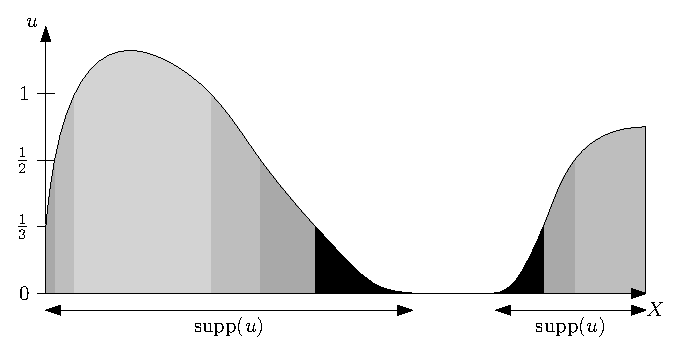
\includegraphics[width=0.75\linewidth]{img/degiorgi.eps}
        \caption{Schematic illustration on how to probe for the support in the proof of De Giorgis theorem: We construct the support by subsequently finding the points \(x \in X\) with \(u(x) \geq 1/n\) for \(n \in \mathbb{N}_{\geq 1}\).}
        \label{fig:degiorgi_decomposition_illustration}
    \end{figure}

    \begin{figure}[!hbtp]
        \centering
        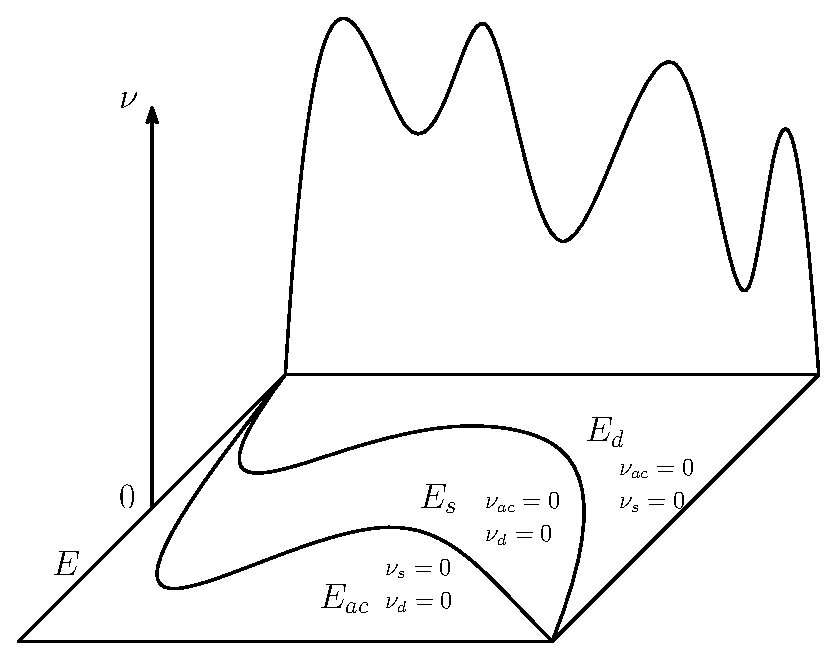
\includegraphics[width=0.4\linewidth]{img/degiorgi2.eps}
        \caption{General illustration of the partition found in the proof of De Giorgis theorem.}
        \label{fig:degiorgi_decomposition_illustration_2}
    \end{figure}

    \section{Decomposition Theorems for Signed Measures}

    In the same manner as for general measures, we can study decompositions of signed measures.

    \subsection{Signed Measures}

    \begin{definition} \label{def:signed_measures}
        A function \(\lambda\colon \mathfrak{M} \to [-\infty, \infty]\) is called a \emph{signed measure}, if:
        \begin{enumerate}[label=(\roman*)]
            \item \(\lambda(\emptyset) = 0\)
            \item \(|\{-\infty, \infty\} \cap \text{im}(\lambda)| \leq 1\)
            \item For any mutually disjoint family \(\{E_n \subseteq \mathfrak{M}\}_{n \in \mathbb{N}_{\geq 1}}\), we have \(\lambda\left(\bigcup_{n=1}^\infty E_n\right) = \sum_{n=1}^\infty \lambda(E_n)\).
        \end{enumerate}
    \end{definition}

    In the following, \(\lambda\) will denote a signed measure according to \Cref{def:signed_measures}. Consider the following characterization.

    \begin{lemma} \label{lem:limit_characterization_of_signed_measures}
        A set function \(\lambda\colon \mathfrak{M} \to [-\infty, \infty]\) is a signed measure, iff it satisfies the following:
        \begin{enumerate}[label=(\roman*)]
            \item \(|\{-\infty, \infty\} \cap \text{im}(\lambda)| \leq 1\)
            \item \(\lambda(E \cup F) = \lambda(E) + \lambda(F)\) for disjoint \(E, F \in \mathfrak{M}\).
            \item For any increasing sequence \(\{E_n \subseteq \mathfrak{M}\}_{n \in \mathbb{N}_{\geq 1}}\), we have \(\lambda\left(\bigcup_{n=1}^\infty E_n\right) = \lim_{n \to \infty} \lambda(E_n)\).
        \end{enumerate}
    \end{lemma}

    \begin{proof}
        \((\Rightarrow)\) We only have to consider the third point. Let \(\{E_n \in \mathfrak{M}\}_{n \in \mathbb{N}_{\geq 1}}\) be an increasing sequence. Set \(F_1 \coloneqq E_1\) and
        \begin{align}
            F_n \coloneqq E_n \setminus E_{n-1}
        \end{align}
        for \(n \in \mathbb{N}_{\geq 2}\). Then
        \begin{align}
            \lambda\left(\bigcup_{n=1}^\infty E_n\right) = \lambda\left(\bigcup_{n=1}^\infty F_n\right) = \sum_{n=1}^\infty \lambda(F_n) = \lim_{n \to \infty} \sum_{i=1}^n \lambda(F_i) = \lim_{n \to \infty} \lambda\left(\bigcup_{i=1}^n F_i\right) = \lim_{n \to \infty} \lambda(E_n).
        \end{align}

        \((\Leftarrow)\) We first have \(\lambda(\emptyset) = \lambda(\emptyset \cup \emptyset) = 2\lambda(\emptyset)\), from which we get \(\lambda(\emptyset) = 0\). Second, let \(\{F_n\}_{n \in \mathbb{N}_{\geq 1}} \subseteq \mathfrak{M}\) be some mutually disjoint family. Define for any \(n \in \mathbb{N}_{\geq 1}\)
        \begin{align}
            E_n \coloneqq \bigcup_{k=1}^n F_k.
        \end{align}
        Then we have
        \begin{align}
            \lambda\left(\bigcup_{k=1}^\infty F_k\right) = \lambda\left(\bigcup_{n=1}^\infty E_n\right) = \lim_{n \to \infty} \lambda(E_n) = \lim_{n \to \infty} \sum_{k=1}^n \lambda(F_k) = \sum_{k=1}^\infty \lambda(F_k).    
        \end{align}
    \end{proof}

    \subsection{Positive/Negative Sets and the Hahn Decomposition Theorem}

    \begin{definition}
        A set \(E \in \mathfrak{M}\) is called \emph{positive}, if \(\lambda(F) \geq 0\), and resp. \emph{negative}, if \(\lambda(F) \leq 0\), for all \(\mathfrak{M} \ni F \subseteq E\).
    \end{definition}

    We wish to prove a finiteness lemma for proving the existence of a positive subset. We then follow these lemmas up with the first decomposition theorem for signed measures, which directly connects to the notion of positive and negative sets.

    \begin{lemma} \label{lem:finiteness_lemma}
        Let \(E \in \mathfrak{M}\) with \(|\lambda(E)| < \infty\). Then for any \(\mathfrak{M} \ni F \subseteq E\), \(|\lambda(F)| < \infty\).
    \end{lemma}

    \begin{proof}
        Wlog. suppose \(\text{im}(\lambda) \subseteq [-\infty, \infty)\), where the other case is analogous. If \(\lambda(F) \geq 0\), we are done. Else,
        \begin{align}
            0 < -\lambda(F) = -(\lambda(E \setminus F) + \lambda(F) - \lambda(E \setminus F)) = \lambda(E \setminus F) - \lambda(E) < \infty,
        \end{align}
        where the latter inequality comes from the fact, that \(\infty \notin \text{im}(\lambda)\) and \(|\lambda(E)| < \infty\), giving the statement.
    \end{proof}

    \begin{edgebox}
        \begin{lemma}[{\cite[pp. 59-60]{Fonseca}}] \label{lem:supremum_lemma}
            Let \(\mu\colon \mathfrak{M} \to [0, \infty)\) be a finite measure. Define:
            \begin{align}
                \mu^+\colon \mathfrak{M} \to [0, \infty), E \mapsto \sup\{\mu(E') \mid \mathfrak{M} \ni E' \subseteq E\}
            \end{align}
            \begin{enumerate}[label=(\roman*)]
                \item \(\mu^+\) is well-defined and a measure.
                \item For any \(E \in \mathfrak{M}\), we have:
                \begin{align}
                    \mu^+(E) = \sup\{\mu(E') \mid \mathfrak{M} \ni E' \subseteq E, (-\mu)^+(E') = 0\}
                \end{align}
            \end{enumerate}
        \end{lemma}
    \end{edgebox}

    For the sake of time, as its proof is quite long and rather tedious, we skip the proof of \Cref{lem:supremum_lemma}. In the following, we adapt the restriction notation for measures to signed measures: If \(E \in \mathfrak{M}\) and \(\lambda\colon \mathfrak{M} \to [-\infty, \infty]\) is a signed measure, then \(\lambda|_E\colon \mathfrak{M}|_E \to [-\infty, \infty], F \mapsto \lambda(F \cap E)\) is a natural signed measure.

    \begin{lemma} \label{lem:existence_of_positive_subset}
        Let \(E \in \mathfrak{M}\) with \(\lambda(E) \in (0, \infty)\). Then there exists a positive \(\mathfrak{M} \ni F \subseteq E\).
    \end{lemma}

    \begin{proof}
        By \Cref{lem:finiteness_lemma}, \(\lambda|_E\) is finite. Define:
        \begin{align}
            \lambda_+&\colon \mathfrak{M}|_E \to [0, \infty), F \mapsto \sup\{\lambda(F') \mid \mathfrak{M} \ni F' \subseteq F\}\\
            \lambda_-&\colon \mathfrak{M}|_E \to [0, \infty), F \mapsto -\inf\{\lambda(F') \mid \mathfrak{M} \ni F' \subseteq F\}
        \end{align}
        Then by \Cref{lem:supremum_lemma}, \(\lambda_+\) and \(\lambda_-\) are finite measures. Furthermore, since
        \begin{align}
            \lambda_+(E) &= \sup\{\lambda(E') \mid \mathfrak{M} \ni E' \subseteq E, \lambda_-(E') = 0\}\\
            &= \sup\{\lambda(E') \mid \mathfrak{M} \ni E' \subseteq E, E' \text{ positive}\}
        \end{align}
        and \(\lambda(E) \in (0, \infty)\), there exists a positive subset \(E' \subseteq E\), giving the statement.
    \end{proof}

    % \begin{lemma}[{...}] % Elstrodt? -> Do not need some more explicit argument for construction.
    %     Let \(E \in \mathfrak{M}\). ...
    % \end{lemma}

    \begin{theorem}[Hahn Decomposition Theorem] \label{thm:hahn_decomposition}
        Any measurable space \((X, \mathfrak{M})\) can be decomposed as \(X = X^+ \cup X^-\), where \(X^+ \subseteq X\) is positive and \(X^- \subseteq X\) is negative.
    \end{theorem}

    \begin{proof}
        Wlog. suppose \(\text{im}(\lambda) \subseteq [-\infty, \infty)\). Let
        \begin{align}
            \Xi \coloneqq \sup\{\lambda(E) \mid E \in \mathfrak{M} \text{ positive}\}.
        \end{align}
        As this is a supremum, we may take a sequence \((E_n' \in \mathfrak{M})_{n \in \mathbb{N}_{\geq 1}}\) with \(\lim_{n \to \infty} \lambda(E_n') = \Xi\) and define \((E_n \coloneqq \bigcup_{m=1}^n E_m')_{n \in \mathbb{N}_{\geq 1}}\) to be its canonical associated increasing sequence of positive sets, also fulfilling
        \begin{align}
            \lim_{n \to \infty} \lambda(E_n) = \Xi.
        \end{align}
        Define
        \begin{align}
            X^+ \coloneqq \bigcup_{n=1}^\infty E_n.
        \end{align}
        Then \(X^+\) is positive by definition and
        \begin{align}
            \lambda(X^+) = \lim_{n \to \infty} \lambda(E_n) = \Xi,
        \end{align}
        because of \Cref{lem:limit_characterization_of_signed_measures}. We claim, that \(X^- \coloneqq X \setminus X^+\) is negative. If not, then there is an \(\mathfrak{M} \ni F \subseteq X^-\) with \(\lambda(F) \in (0, \infty)\). By \Cref{lem:existence_of_positive_subset}, there is a positive \(\mathfrak{M} \ni F' \subseteq F\) with \(\lambda(F') > 0\), but then
        \begin{align}
            \Xi = \lambda(X^+) < \lambda(X^+) + \lambda(F') = \lambda(X^+ \cup F') < \infty,
        \end{align}
        thus \(\Xi < \lambda(X^+ \cup F')\), although \(F'\) is positive \lightning. The proof can be done analogously for the case \(\lambda(X) \subseteq (-\infty, \infty]\) by first constructing \(X^-\) using negativity and then proceeding analogously.
    \end{proof}

    We may interpret \Cref{thm:hahn_decomposition} as a decomposition of a signed measure, as the theorem gives the possibility of decomposing a space wrt. the \emph{action} of a signed measure. Elstrodt \cite[p. 271]{Elstrodt} gives the interpretation of the Hahn decomposition as a differentiation between the \emph{charges} of \(\lambda\) over \(X\), as depicted in \Cref{fig:hahn_decomposition_illustration}.

    \begin{figure}[!hbtp]
        \centering
        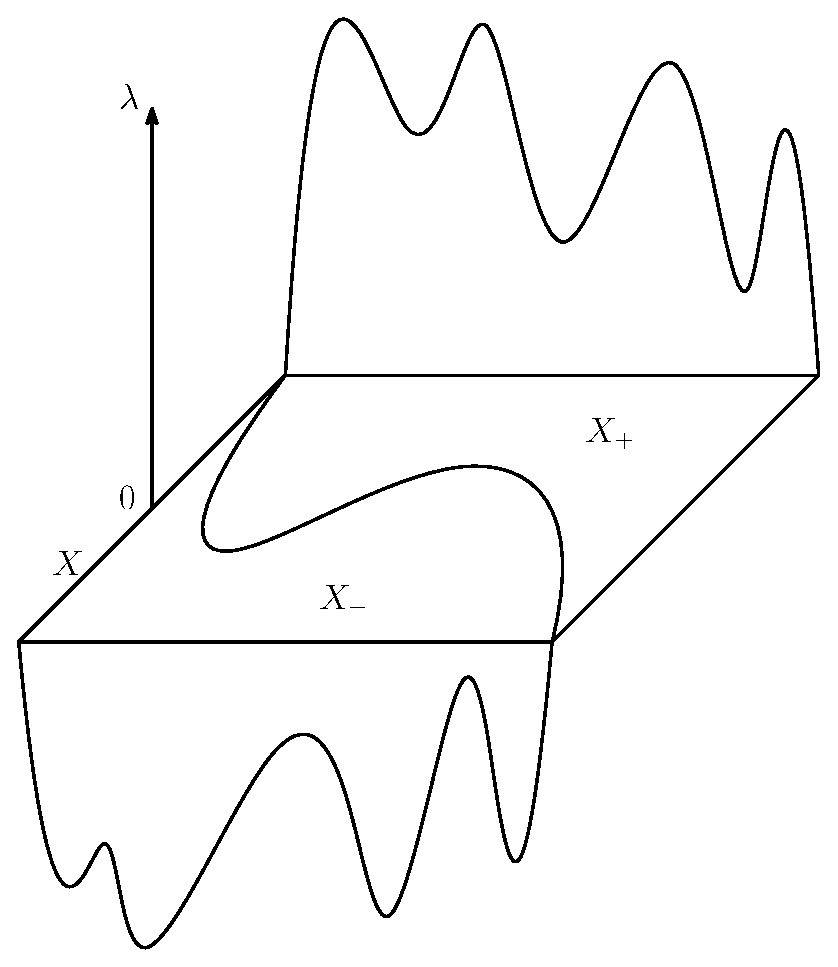
\includegraphics[width=0.4\linewidth]{img/hahn.eps}
        \caption{Schematic Illustration of the Hahn decomposition theorem.}
        \label{fig:hahn_decomposition_illustration}
    \end{figure}

    \begin{remark}
        In general, the Hahn decomposition is not unique. Let \(X = [-1, 1]\), \(\mathfrak{M} = \mathcal{B}([-1, 1])\) and
        \begin{align}
            \lambda(E) \coloneqq \int_E x \, dx \text{ for } E \in \mathfrak{M}.
        \end{align}
        Then \(([0, 1], [-1, 0))\) and \(((0, 1], [-1, 0])\) are both Hahn decompositions of \(X\).
    \end{remark}

    \subsection{The Jordan and Lebesgue Decomposition Theorems}

    Using Hahn decomposition theorem to decompose the action of \(\lambda\) wrt. \(X^+\) and \(X^-\), we arrive at the following result.

    \begin{theorem}[Jordan Decomposition Theorem] \label{thm:jordan_decomposition}
        There exists a unique pair \((\lambda^+, \lambda^-)\) of measures with \(\lambda^+ \perp \lambda^-\), one being finite and \(\lambda = \lambda^+ - \lambda^-\).
    \end{theorem}

    \begin{proof}
        Apply \Cref{thm:hahn_decomposition} on \(X\) to obtain \((X^+, X^-)\) and set the restriction measures \(\lambda^+ \coloneqq \lambda|_{X^+}\) and \(\lambda^- \coloneqq -\lambda|_{X^-}\). By construction, \(\lambda^+ \perp \lambda^-\) and \(\lambda = \lambda^+ - \lambda^-\). As for the uniqueness, we use the argument given by Axler \cite[p. 269]{Axler}: We have \(\lambda = \lambda^+ - \lambda^-\) and \(|\lambda| = \lambda^+ + \lambda^-\), giving
        \begin{align}
            \lambda^+ = \frac{|\lambda|+\lambda}{2} \text{ and } \lambda^- = \frac{|\lambda|-\lambda}{2},
        \end{align}
        so \(\lambda^+\) and \(\lambda^-\) are uniquely determined by \(\lambda\) itself.
    \end{proof}

    \begin{remark}[Justification of the Lebesgue Integral]
        In light of the Jordan decomposition theorem, we can give a more abstract justification for the definition of the Lebesgue integral: Let \(u\colon X \to [-\infty, \infty]\) be a measurable function and \(E \in \mathfrak{M}\). If either \(\int_E u \, d\lambda^+\) or \(\int_E u \, d\lambda^-\) is finite, then we can define the Lebesgue integral as
        \begin{align}
            \int_E u \, d\lambda \coloneqq \int_E u \, d\lambda^+ - \int_E u \, d\lambda^-
        \end{align}
        in the same manner as if we were to Jordan decompose the signed measure \(E \mapsto \int_E u \, d\lambda\), in case of \(u\) being Lebesgue integrable.
    \end{remark}

    For the following, we generalize some of the basic definitions seen in \Cref{def:basic_definitions} directly to signed measures.

    \begin{definition}
        Let \((\lambda^+, \lambda^-), (\varsigma^+, \varsigma^-)\) be the Jordan decompositions of signed measures \(\lambda, \varsigma\colon X \to [-\infty, \infty]\).
        \begin{enumerate}[label=(\roman*)]
            %\item \(E \in \mathfrak{M}\) is said to have \(\sigma\)-finite measure \(\lambda\), if it has \(\sigma\)-finite measure \(\lambda^++\lambda^-\).
            %\item \(\lambda\) is said to be \(\sigma\)-finite, if \(X\) has \(\sigma\)-finite measure \(\lambda\).
            \item \(\lambda\) is said to be \emph{absolutely continuous wrt. \(\varsigma\)}, written \(\lambda \ll \varsigma\), if \(\lambda^++\lambda^- \ll \varsigma^++\varsigma^-\).
            \item \(\lambda\) and \(\varsigma\) are said to be \emph{mutually singular}, written \(\lambda \perp \varsigma\), if \(\lambda^++\lambda^- \perp \varsigma^+ + \varsigma^-\).
        \end{enumerate}
    \end{definition}

    The culmination of the decomposition theorems presented lies in the following theorem.

    \begin{theorem}[Signed Lebesgue Decomposition Theorem]
        Let \(\lambda\colon \mathfrak{M} \to [-\infty, \infty]\) be a signed measure and \(\mu\colon \mathfrak{M} \to [0, \infty]\) be a \(\sigma\)-finite measure.
        \begin{enumerate}[label=(\roman*), wide]
            \item \label{thm:lebesgue_decomposition_thm_1} There are signed measures \(\lambda_{ac}, \lambda_s\colon X \to [-\infty, \infty]\) and a measurable function \(u\colon X \to [-\infty, \infty]\) with
            \begin{align}
                \lambda = \lambda_{ac} + \lambda_s,
            \end{align}
            \(\lambda_{ac} \ll \mu\) and
            \begin{align}
                \lambda_{ac}(\cdot) = \int_{\cdot} u \, d\mu.
            \end{align}
            \item \label{thm:lebesgue_decomposition_thm_2} If \(\lambda\) is \(\sigma\)-finite, then \(\lambda_s \perp \mu\) and the decomposition is unique.
        \end{enumerate}
    \end{theorem}

    We recall, that the measurability of \(u\) is to be understood wrt. the associated canonical Borel algebra of \([-\infty, \infty]\).

    \begin{proof}
        \ref{thm:lebesgue_decomposition_thm_1} Apply \Cref{thm:jordan_decomposition} and \Cref{thm:lebesgue_decomposition_theorem} twice to obtain
        \begin{align}
            \lambda = \lambda^+ + \lambda^-, \lambda^+ = \lambda^+_{ac} + \lambda^+_s \text{ and } \lambda^- = \lambda^-_{ac} + \lambda^-_s
        \end{align}
        with \(\lambda^+_{ac}, \lambda^-_{ac} \ll \mu\). Applying \Cref{thm:radon_nikodym_i} twice then gives measurable \(u^+, u^-\colon X \to [0, \infty]\) with
        \begin{align}
            \lambda^+_{ac}(\cdot) = \int_\cdot \, u^+ \, d \mu \text{ and } \lambda^-_{ac}(\cdot) = \int_\cdot \, u^- \, d \mu.
        \end{align}
        Either \(\lambda^+\) or \(\lambda^-\) or none are finite, so we can define
        \begin{align}
            \lambda_{ac} \coloneqq \lambda^+_{ac} - \lambda^-_{ac}, \lambda_s \coloneqq \lambda^+_s - \lambda^-_s \text{ and } u \coloneqq u^+ - u^-,
        \end{align}
        the first two of which are signed measures. Especially, \(\lambda_{ac} \ll \mu\) and if \(\lambda\) is positive, so are \(\lambda_{ac}\) and \(\lambda_s\) by construction. This gives the statement.

        \ref{thm:lebesgue_decomposition_thm_2} The singularity and uniqueness follows from the construction in \ref{thm:lebesgue_decomposition_thm_1}.
    \end{proof}

    \section{Summary} \phantom{}

    For the end of these notes, we summarize some major decomposition theorems in \cite[pp. 1-119]{Fonseca}, including those discussed. Here, \(\mu_p\) denotes a purely finitely additive measure \cite[p. 8]{Fonseca}, \(\mu_c\) denotes a countably additive measure \cite[p. 5]{Fonseca} and \(\mu_1\) and \(\mu_2\) denote atomatic and non-atomic measures \cite[p. 10]{Fonseca}.

    \phantom{}

    \begin{minipage}{\linewidth}
        \centering
        \begin{tabular}{C{4cm}|C{3cm}}
            Decomposition & Summary \\\hline
            Hewitt-Yosida \cite[pp. 8-9]{Fonseca} & \(\mu = \mu_p + \mu_c\)\\
            Atomic \cite[pp. 13-16]{Fonseca} & \(\mu = \mu_1 + \mu_2\)\\
            Lebesgue & \(\nu = \nu_{ac} + \nu_s\)\\
            De Giorgi & \(\nu = \nu_{ac} + \nu_s + \nu_d\)\\
            Hahn & \(X = X^+ \cup X^-\)\\
            Jordan & \(\lambda = \lambda^+ - \lambda^-\)\\
            Signed Lebesgue & \(\lambda = \lambda_{ac} + \lambda_s\)
        \end{tabular}
    \end{minipage}

    \printbibliography{}
\end{document}
